\pdfvariable minorversion=7
\pdfvariable inclusioncopyfonts=1

\documentclass{arialFHGR} % use either arialFHGR or timesFHGR
\newcommand{\haupttitel}{Proposal Masterthesis}
\newcommand{\untertitel}{Interaktive Visualisierung dynamischer Netzwerke - Implementierung eines Visual Analytics Tools zur Exploration von Anomalien und Trends im SBB Zugverkehrsnetzwerk}
\newcommand{\zusammenfassung}{Abstract}
\newcommand{\autorenschaft}{Yannick Hutter}
\newcommand{\studiengang}{Msc User Experience Design \& Data Visualization}
\newcommand{\matrikelnummer}{17-175-829}
\newcommand{\adresse}{Talackerstrasse 8}
\newcommand{\ort}{Mels}
\newcommand{\plz}{8887}
\newcommand{\department}{[Departement]}
\newcommand{\institute}{[Institutsname]}
\newcommand{\modul}{Masterthesis FS25}
\newcommand{\email}{yannick.hutter@stud.fhgr.ch}
\newcommand{\refe}{Dr. rer. nat Michael Burch}
\newcommand{\coRefe}{Prof. Dr. habil. Wolfgang Semar}
\newcommand{\abgabedatum}{02.05.2025}
\newcommand{\abgabedatumRFC}{2025-05-02}
\newcommand{\sprache}{de}
\newcommand{\schlagworte}{}

\usepackage{setspace, fancyhdr, lscape, floatrow, caption, inputenc, graphicx, enumitem, tabularx, colorprofiles, xstring, hyphenat, chngcntr, xspace, listings, pdfpages}

\usepackage[left=3cm,right=2.5cm,top=2.5cm,bottom=2cm]{geometry}
\usepackage[backend=biber,style=apa,citestyle=apa]{biblatex}
\usepackage[autostyle]{csquotes}
\usepackage[english, nswissgerman]{babel}
\usepackage[titles]{tocloft}
\usepackage[hang,flushmargin]{footmisc}

% Settings for glossary
\usepackage[acronym,toc=true,xindy,nopostdot=true,nonumberlist,nogroupskip=true]{glossaries}
\loadglsentries{content/01_vorspann/01.4_abkuerzungsverzeichnis_glossar}
\setglossarystyle{alttree}
\setglossarypreamble[acronym]{\vspace*{-8pt}}
\makeglossaries
\glsaddall
\glsfindwidesttoplevelname

\graphicspath{{content/00_assets}} % Set path as default for including graphics
\addbibresource{content/00_assets/quellen.bib} % Add bibliography entries

% cite with acronym. 
% Example input: \citeAbbr{schweizerische_archivdirektorinnen-_und_archivdirektorenkonferenz_informations-_2018}{adk}
\newcommand{\parenciteabbr}[2]{(\acrlong{#2} [\acrshort{#2}], \citeyear{#1})}
\newcommand{\textciteabbr}[2]{\acrlong{#2} (\acrshort{#2}, \citeyear{#1})}
\newcommand{\acrfullSqBr}[1]{\acrlong{#1} [\acrshort{#1}]}

\setmonofont{Courier New}

% Settings for listings
\lstdefinestyle{codeStyle}{
    belowcaptionskip=6pt,
    belowskip=3pt,
    breaklines=true,
    numbers=left,
    basicstyle=\footnotesize\ttfamily,
    extendedchars=true,
    frame=single,
    captionpos=t,
    numberbychapter=false,
    xleftmargin=4pt,
    xrightmargin=4pt
}
\lstset{style=codeStyle}

% Settings for blockquote
\SetBlockEnvironment{quotation}
\patchcmd{\quotation}{\rightmargin}{\leftmargin 1.3cm \rightmargin 0}{}{}
\NewCommandCopy{\oldblockquote}{\blockquote}
\renewcommand{\blockquote}[1]{\oldblockquote{\noindent #1}}

% Settings for figure and table
\counterwithout{figure}{chapter}
\counterwithout{table}{chapter}

\floatsetup[figure]{
    capposition=above,
    captionskip=2pt
}

\DeclareCaptionLabelFormat{figTitle}{%
    Abbildung \the\numexpr\value{figure}\relax\\
}

\captionsetup[figure]{
    font={normalsize,stretch=1.0},
    labelfont=bf,
    labelsep=none,
    labelformat=figTitle,
    textfont=it,
    justification=raggedright,
    singlelinecheck=false,
    position=above,
}

\floatsetup[table]{
    capposition=above,
    captionskip=2pt
}

\DeclareCaptionLabelFormat{tabTitle}{%
    Tabelle \the\numexpr\value{table}\relax \\
} 

\captionsetup[table]{
    font={normalsize,stretch=1.0},
    labelfont={bf},
    labelsep=none,
    labelformat=tabTitle,
    textfont=it,
    justification=raggedright,
    singlelinecheck=false,
    position=above
}

\floatsetup[lstlisting]{
    capposition=above,
    captionskip=2pt
}

\DeclareCaptionLabelFormat{codeTitle}{%
    Programmcode \the\numexpr\value{lstlisting}\relax \\
} 

\captionsetup[lstlisting]{
    font={normalsize,stretch=1.0},
    labelfont={bf},
    labelsep=none,
    labelformat=codeTitle,
    textfont=it,
    justification=raggedright,
    singlelinecheck=false,
    position=above
}

\renewcommand{\thetable}{\arabic{table}}
\renewcommand{\thefigure}{\arabic{figure}}

% Einstellungen für tocloft / Settings for tocloft
\renewcommand{\cftfigpresnum}{Abb.~}
\renewcommand{\cfttabpresnum}{Tab.~}
\renewcommand{\cftfigaftersnum}{:}
\renewcommand{\cfttabaftersnum}{:}
\setlength{\cftfignumwidth}{2cm}
\setlength{\cfttabnumwidth}{2cm}
\setlength{\cftfigindent}{0cm}
\setlength{\cfttabindent}{0cm}

\setstretch{1.3} % Zeilenabstand / line spacing
\renewcommand{\arraystretch}{1.3} % Zeilenabstand innerhalb von Tabellen / line spacing in tables
\setlength{\parindent}{1.3cm} % Einzug neuer Absatz / Indentation new paragraph
\fancyhf{}
\renewcommand{\headrulewidth}{0pt}
\pagestyle{fancyplain}
\rfoot{\footnotesize\thepage}

\usepackage[pdfa]{hyperref}
\usepackage{hyperxmp}
\usepackage{embedfile}
\pdfvariable omitcidset=1

% 
\newcommand{\chapterNoNr}[1]{%
    \chapter*{#1}
    \addcontentsline{toc}{chapter}{#1} %
}%

\newcommand{\note}[1]{%
    \doublespacing\raggedright\footnotesize{\textit{Anmerkung:} #1}
}%

\newcommand{\sic}{%
    [\textit{sic}]\xspace
}%

\makeatletter
\def\l@lstlisting#1#2{\@dottedtocline{1}{0em}{2em}{Programmcode #1}{#2}}
\makeatother

\hypersetup{%
    pdflang=\sprache,
    pdftitle={\haupttitel},
    pdfsubtitle={\untertitel},
    pdfauthor={\autorenschaft},
    pdfdate={\abgabedatumRFC},
    pdfsubject={\zusammenfassung},
    pdfkeywords={\modul, \schlagworte},
    pdfcontactaddress={\adresse},
    pdfcontactcity={\ort},
    pdfcontactpostcode={\plz},
    pdfcontactemail={\email},
    colorlinks,
    unicode,
    allcolors=black,
    pdfapart=2,
    pdfaconformance=U
}

% 
\immediate\pdfobj stream attr{/N 3} file{sRGB.icc}
\pdfcatalog{%
  /OutputIntents [
    <<
      /Type /OutputIntent
      /S /GTS_PDFA1
      /DestOutputProfile \the\pdflastobj\space 0 R
      /OutputConditionIdentifier (sRGB)
      /Info (sRGB)
    >>
  ]
}

\begin{document}

    \renewcommand{\contentsname}{Inhaltsverzeichnis}
    \renewcommand{\listfigurename}{Abbildungsverzeichnis}
    \renewcommand{\listtablename}{Tabellenverzeichnis}
    \renewcommand{\acronymname}{Abkürzungsverzeichnis}
    \renewcommand{\lstlistlistingname}{\texorpdfstring{Programmcodeverzeichnis\bigskip}{Programmcodeverzeichnis}}
    
    % Start Vorspann
    
    \pagenumbering{Roman} % Begin roman pagenumbering

    % Titelblatt für eine Studienarbeit
     \begin{titlepage}
    
    \begin{center}
        Geschrieben an der Fachhochschule Graubünden \\
        \vspace{30mm}
        \huge\textbf{\haupttitel}\\
        \hfill \break
        \large{(\untertitel)}
    \end{center}
    
    \vfill
    
    \begin{flushleft}
    Name: \autorenschaft\\
    Studiengang: \studiengang\\
    Matrikelnummer: \matrikelnummer\\
    Adresse: \adresse, \plz~\ort\\
    E-Mail: \email\\
    ~\\
    Modul: \modul\\
    Referent: \refe\\
    Koreferent: \coRefe\\
    ~\\
    Abgabedatum: \abgabedatum
    \end{flushleft}
    
    \vspace{20mm}
    
\end{titlepage}

    % ODER für eine Abschlussarbeit
    % \begin{titlepage}
    \begin{center}
        {\large
            {\Large\textbf{\haupttitel}} \\
            \textit{\untertitel} \\
            ~\\
            An der Fachhochschule Graubünden \\
            \department \\
            \institute \\
            \vspace{2mm}
            im Studiengang \studiengang{} eingereichte \\
            ~\\
            {\Huge\textbf{Masterarbeit}} \\
            ~\\
            zur Erlangung des akademischen Grades \\
            eines Master of Science (M.Sc.)
    
            \vspace{40mm}
            vorgelegt von \\
            \vspace{4mm}
            {\Large\textbf{\autorenschaft}} \\
            \vspace{4mm}
            Matrikelnr.: \matrikelnummer \\
            E-Mail: \email \\
            ~\\~\\
            Erstgutachter: \refe \\
            Zweitgutachter: \coRefe \\
            ~\\
            Eingereicht am: \abgabedatum
        } % end large
    \end{center}
\end{titlepage}


    \include{content/01_vorspann/01.2_abstract}
    \include{content/01_vorspann/01.3_vorwort}

    \tableofcontents % Inhaltsverzeichnis
        
    % List of figures
    \cleardoublepage
    \phantomsection
    \addcontentsline{toc}{chapter}{\listfigurename}
    \listoffigures
    
    % List of tables
    \cleardoublepage
    \phantomsection
    \addcontentsline{toc}{chapter}{\listtablename}
    \listoftables

    % List of acronyms
    \printglossary[type=\acronymtype]
    \cleardoublepage
    \newpage
    % Ende Vorspann
    
    % Start Textteil
    \pagenumbering{arabic} % Begin arabic pagenumbering
    \include{content/02_textteil/einleitung}
    \chapter{Forschungsproblem und Forschungsziel}
\label{kap:forschungsproblem_forschungsziel}
Schweizer fahren gerne Zug, dies zeigt ein Artikel von Litra, welcher die Nutzung des Zuges in Europa untersuchte \parencite{litra_bahnfahrtstatistik_europa_2023}. Alleine im Jahr 2023 legten die Schweizer rund 2'466 Bahnkilometer pro Einwohner zurück (siehe Abbildung \ref{fig_schweizer_fahren_zug}). Dies entspricht einem Zuwachs von rund 13 Prozent im Vergleich zum Vorjahr. 

\begin{figure}[H]
    \caption{Zurückgelegte Kilometer pro Einwohnerin und Einwohner 2023 (Personenkilometer) \parencite{litra_bahnfahrtstatistik_europa_2023}}
    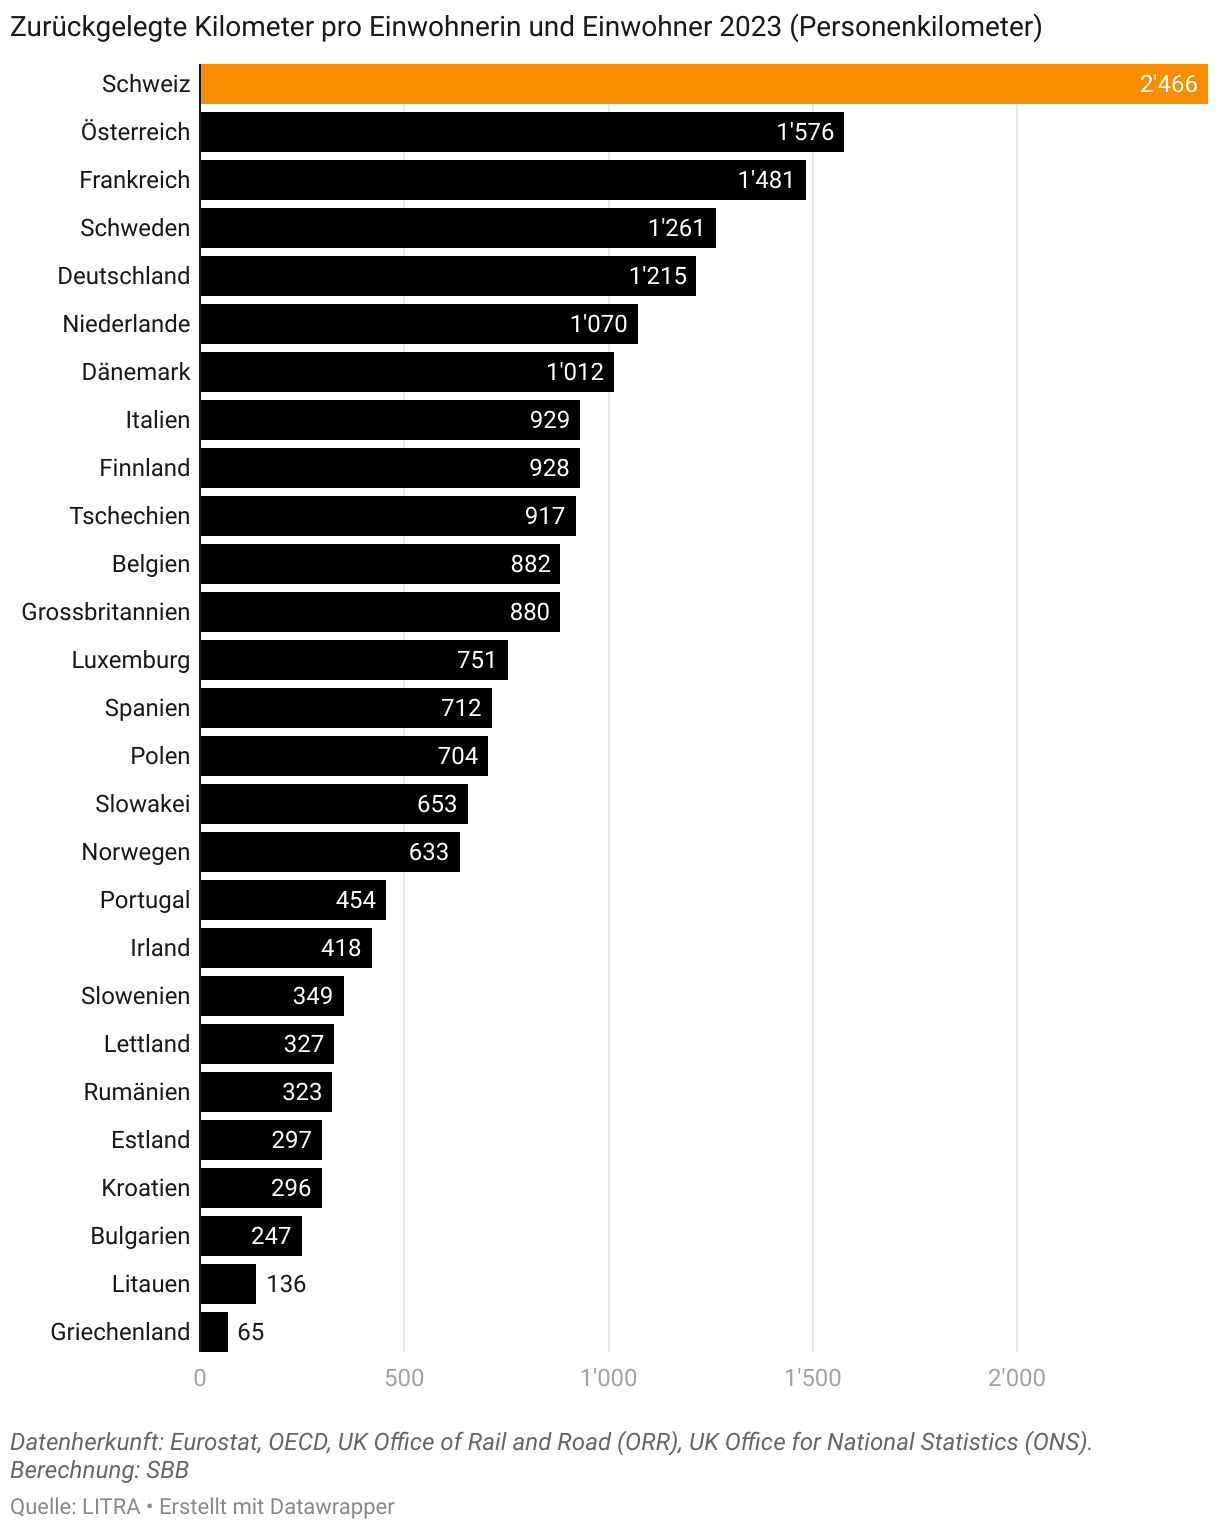
\includegraphics[width=.4\linewidth]{content/00_assets/schweizer_fahren_zug.png}
    \label{fig_schweizer_fahren_zug}
\end{figure}

Auch scheint es keine Anzeichen einer Abschwächung der Zugnutzung zu geben, ganz im Gegenteil. Gemäss der \acrfull{sbb} sollen im Jahr 2040 bereits zwei Millionen Menschen pro Tag mit dem Zug fahren, dies entspricht einer Zunahme von rund 30 Prozent \parencite{sbb_ausbauschritt_2025}.

Schaut man sich die Zahlen und Fakten für das SBB-Zugverkehrsnetz aus dem Jahr 2024 an, ergeben sich beachtliche Werte. Täglich werden rund 1.4 Millionen Menschen mithilfe von 11'569 Zügen transportiert. Um das Zugnetz der SBB auf Stand zu halten, werden rund 20'000 Baustellen pro Jahr betrieben. Um es mit den Worten der SBB auszudrücken, sind sowohl das Bauen als auch das Fahren eine Herausforderung \parencite[S.8 - 9]{sbb_geschäftsbericht_2024}. Insbesondere das Fahren nicht nur eine Herausforderung für die Zugnetzbetreiber, sondern auch für die Passagiere, primär dann, wenn Verspätungen involviert sind.

Die vorliegende Arbeit hat sich zum Ziel gesetzt, visuelle Muster und Anomalien im SBB-Zugverkehrsnetzwerk zu explorieren. Hierzu soll ein Visual Analytics Tool entworfen werden. Im Fokus der Arbeit stehen primär Zugverspätungen und deren Auswirkungen. Nebst der eigentlichen Visualisierung der Daten sind auch die dahinterliegenden Algorithmen von grosser Bedeutung. Diese sollen dabei helfen, visuelle Muster auf anschauliche Weise zugänglich zu machen.


    % Ende Textteil
    
    % Start Nachspann
    \printbibliography[heading=bibintoc,title={Literaturverzeichnis}]
    \include{content/03_nachspann/hilfsmittelverzeichnis}
    \appendix
    \chapter{Anhang}

    \include{content/03_nachspann/eiderklaerung}
    % Ende Nachspann
    
\end{document}